%%%%%%%%%%%%%%%%%%%%%%%%%%%%%%%%%%%%%%%%%%%%%%%%%%%%%%%%%%%%%%%%%%%%%%%%%%%%%%%%%%%%%%%%%%%%%%%%%%%%%%
%
%   Filename    : appendix_A.tex 
%
%   Description : This file is for including the Research Ethics Documents (delegated as Appendix A) 
%                 
%%%%%%%%%%%%%%%%%%%%%%%%%%%%%%%%%%%%%%%%%%%%%%%%%%%%%%%%%%%%%%%%%%%%%%%%%%%%%%%%%%%%%%%%%%%%%%%%%%%%%%

\chapter{Code Snippets}
\label{sec:appendixa}



% Save the file you want to include in PDF format.
% Uncomment the commant below specifying the correct appendix file. 
%\includepdf[pages=-, scale = 0.9, pagecommand={}, offset = -30 0]{appendixA.pdf}

\noindent\textbf{i. Machine Learning}
\vspace{-0.5cm}

This section displays the key steps in the machine learning analysis by performing feature engineering to create and transform a new dataset, identifying the most significant features through the Kruskal-Wallis Test, applying random undersampling to address the minimal imbalance in the dataset, and conducting five-fold cross-validation to evaluate the model's performance.


\begin{figure}[!htbp]
	\centering
	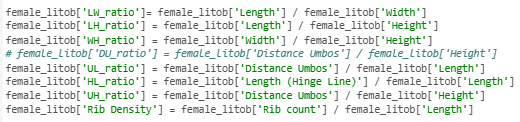
\includegraphics[width=0.9\textwidth, angle=0]{figures/feature_engineering.png}
	\caption{Feature engineering used to create and transform the dataset for machine learning analysis.}
\end{figure}

\begin{figure}[!htbp]
	\centering
	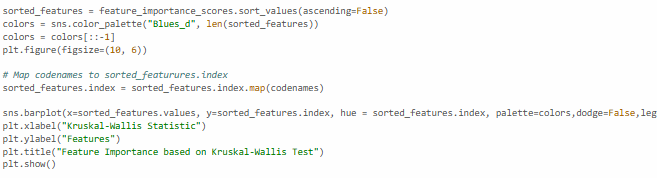
\includegraphics[width=0.9\textwidth, angle=0]{figures/feature_importance.png}
	\caption{Feature importance scores derived from the Kruskal-Wallis test to identify the most significant variables.}
\end{figure}

\begin{figure}[!htbp]
	\centering
	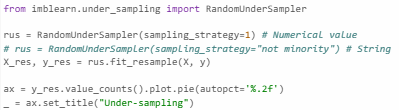
\includegraphics[width=0.9\textwidth, angle=0]{figures/random_undersampling_ML.png}
	\caption{Random undersampling applied in machine learning to address class imbalance.}
\end{figure}

\begin{figure}[!htbp]
	\centering
	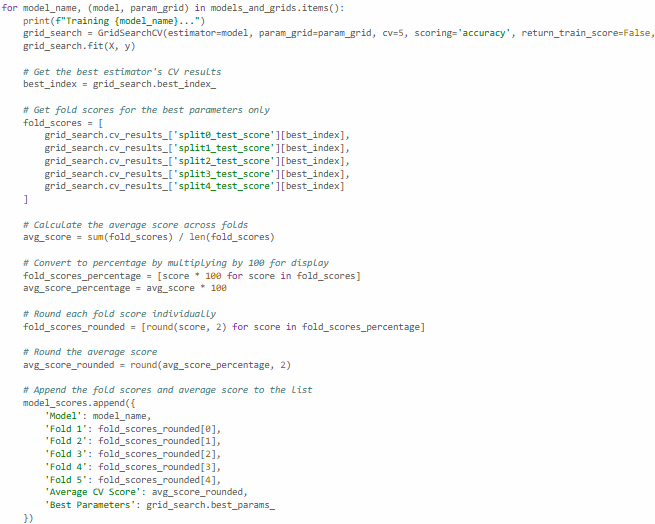
\includegraphics[width=0.9\textwidth, angle=0]{figures/ml_five fold_cv.png}
	\caption{Five-fold cross-validation used to evaluate and tune machine learning model performance.}
\end{figure}

\newpage
\noindent\textbf{ii. Image Processing}
\vspace{-0.5cm}

This section displays the key steps in the image processing by resizing the images to have similar dimensions of 256x256, and the shadows were removed to improve the image quality, and remove noise before proceeding to the deep learning operations.
 
\begin{figure}[!htbp]
	\centering
	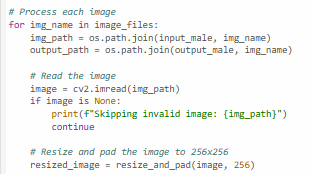
\includegraphics[width=0.9\textwidth, angle=0]{figures/same_dimensions.png}
	\caption{Resizing images to 256x256 pixels for consistent input dimensions.}
\end{figure}

\begin{figure}[!htbp]
	\centering
	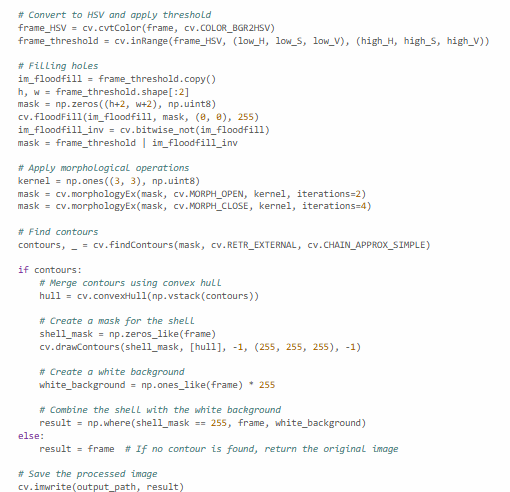
\includegraphics[width=0.9\textwidth, angle=0]{figures/shadow_remove.png}
	\caption{Processing the images to remove the shadows.}
\end{figure}

\newpage

\noindent\textbf{iii. Deep Learning}
\vspace{-0.5cm}

This section outlines the key steps in the deep learning pipeline, including the use of random undersampling to address class imbalance and data augmentation to increase variability in the dataset. The convolutional neural network (CNN) architecture consists of three convolutional layers, followed by a flatten layer and two dense layers. Additionally, early stopping was integrated to halt model training when the validation loss does not improve, and callbacks such as ReduceLROnPlateau were implemented as safeguards against overfitting. ModelCheckpoint was used to save the best model for each fold, allowing the final results to be revisited and analyzed after training; however, it was not heavily utilized in this study.


\begin{figure}[!htbp]
	\centering
	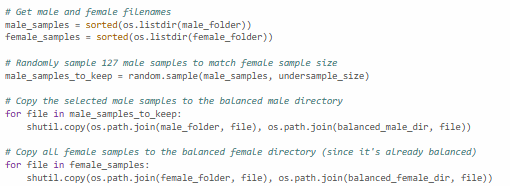
\includegraphics[width=0.9\textwidth, angle=0]{figures/random_undersampling_DL.png}
	\caption{Random undersampling applied in deep learning to balance class distribution in the datasets.}
\end{figure}

\begin{figure}[!htbp]
	\centering
	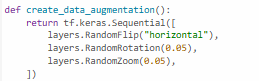
\includegraphics[width=0.9\textwidth, angle=0]{figures/live_augmentation.png}
	\caption{On-the-fly data augmentation used to create a variety of random transformation to increase variation in the training images.}
\end{figure}

\begin{figure}[!htbp]
	\centering
	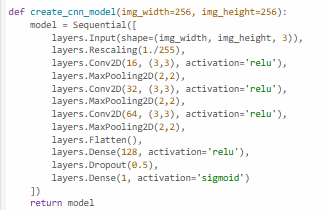
\includegraphics[width=0.9\textwidth, angle=0]{figures/CNN_layers.png}
	\caption{CNN architecture used for training the image dataset.}
\end{figure}

\begin{figure}[!htbp]
	\centering
	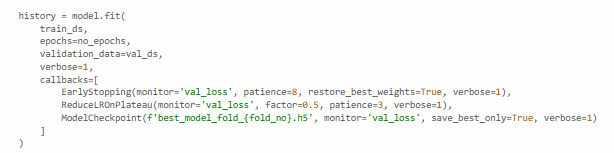
\includegraphics[width=0.9\textwidth, angle=0]{figures/avoid_overfitting.png}
	\caption{Early Stopping and ReduceLROnPlateau used as safeguard against overfitting.}
\end{figure}